\documentclass[letterpaper, 12pt]{article}
\usepackage[american]{babel}
\usepackage[utf8]{inputenc}
\usepackage[citestyle=apa,style=apa,backend=biber]{biblatex}
\usepackage[margin=1in]{geometry}
\usepackage{graphicx}
\usepackage{caption}
\usepackage{float}
\setlength\bibitemsep{2\itemsep}
\DeclareLanguageMapping{american}{american-apa}
\addbibresource{bibliography.bib}

\begin{document}
\begin{titlepage}
\centering
	\vspace*{5.75cm}
	{\huge\bfseries Project proposal\par}
	\vspace{2cm}
	Blair Urish\\
	Dan Wagner\\
	Kansas State University\\
	College of Engineering\\
	Department of Computer Science\\
	\vspace{1cm}
	Dr. Bin Liu\\
	Professor\\
	Department of Chemical Engineering\\
	\vspace{1cm}
	October 29, 2017
\end{titlepage}

\begin{abstract}
\thispagestyle{plain}
\begin{flushleft}
	Abstract goes here if we need it.
\end{flushleft}
\end{abstract}
~\newpage

\begin{flushleft}

\section*{Background Research}
Many fields require materials with properties that often conflict or trade off with one another.  Examples of such properties are low density, high strength, and high flexibility.  In most cases, it is difficult or impossible for traditional materials to exhibit combinations of these properties. Therefore, it is necessary to use hybrid materials that have organic and synthetic components. However, it is difficult to identify these compounds. \cite{C7NR06038F}.\\

Narayanan et. al. discuss two methods of identifying the components needed to create a hybrid material. The first
method discussed is known as the Reactive Force Field (ReaxFF). The authors state that ReaxFF can describe ``bond formation/dissociation, chemical reaction pathways, and transition states in a diverse class of materials.'' However, they note a major issue with ReaxFF: efficiency. ReaxFF requires a large amount of computing power to do its calculations. Many scientists require running simulations with large sample sizes to which ReaxFF does not scale. \\
~\newline
Bond order potentials (BOP) are a different approach that Narayanan et. al. believe could be significantly more
efficient than ReaxFF. They present an approach that combines Tersoff-Brenner modeling with machine learning that
allows for approximations of the attributes needed to describe the hybrid materials mentioned earlier. The goal
with this technique is to provide fairly accurate results compared with ReaxFF. The authors note that
ReaxFF will still be required for certain heterostructures like oxides. \\
~\newline
However, as noted by Dr. Bin Liu, this machine learning algorithm alone is still not performing as well as 
certain scientists require. He believes that it is possible to introduce parallelization to this existing
algorithm in order to further improve performance. In the next section, we will discuss the approach that we
will be taking in order to parallelize this algorithm. 

\section*{Methodology}
 The overall design process can be seen in the following figure.

 \begin{figure}[H]
 	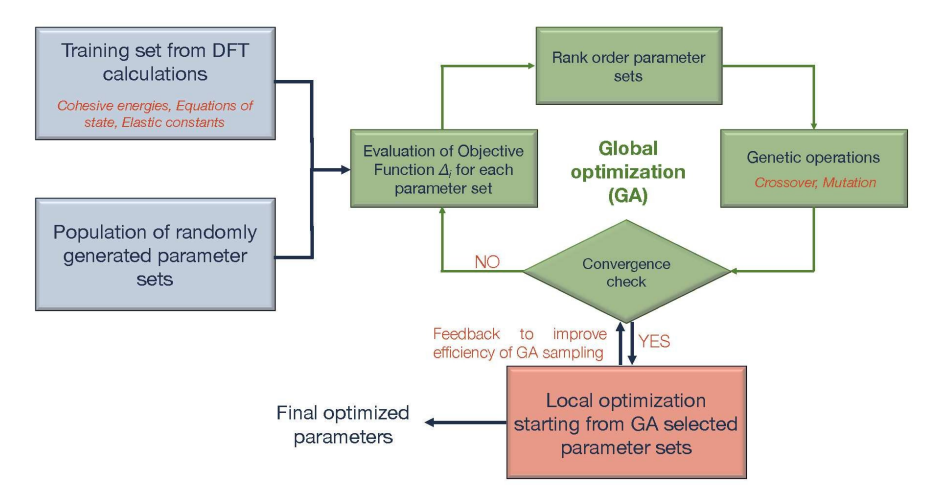
\includegraphics[width=\linewidth,height=10cm,keepaspectratio]{flowchart.png}
 	\caption[Overall Flow of Genetic Algorithm Process]{Overall Flow of Genetic Algorithm Process. Adapted from \cite{C7NR06038F}}
 	\label{fig:arch}
 \end{figure}
 The main optimizations will be taking place within the global optimization loop and the local optimization section, as seen above. The loop will contain the majority of our implementation.  The local optimization section will be carried out primarily with LAMMPS.\\
 
 ~\newline A global single-population master-slave genetic algorithm was chosen as the best method of parallelization. The master node receives a population and divides individuals between the slave nodes.  Slave nodes will evaluate the fitness of individuals they receive and send the results back to the master node.  A visualization of this technique can be seen below.
 
 \begin{figure}[H]
 	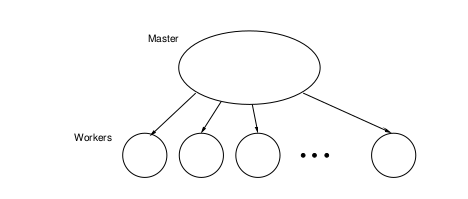
\includegraphics[width=\linewidth,height=10cm,keepaspectratio]{model.png}
 	\caption[Master-Slave Genetic Algorithm Implementation]{Master-Slave Distributed Genetic Algorithm. Adapted from \cite{cantu1998survey}}
 	\label{fig:arch}
 \end{figure}

~\newline We will realize this solution using several nodes on the Beocat supercomputing cluster.   One computing node will be designated as the master node, while several other nodes will be the slave nodes.  The master node will receive the population of randomly generated parameter sets and the training set provided.  It will partition the population into subsets and send the sets to slave nodes for evaluation.  Each slave node will evaluate the fitness of each individual within their subset and transfer the results to the master node for modification via trait crossover and mutation. The best one hundred individuals are retained for subsequent generations.\\

~\newline
This process will continue until the genetic algorithm fails to return better individuals than the previous run.  At this convergence step, the twenty best individuals are selected to be locally minimized by using the Simplex method.  Finally, the most optimized individual results in the best set of parameters for this generation. \\

~\newline The Large-scale Atomic/Molecular Massively Parallel Simulator (LAMMPS) package will be used to evaluate individuals' fitness.  This software is a classical molecular dynamics code developed by Sandia National Laboratories.  It has optimized integrations with MPI, which will fit into our overall design very well.




\section*{Conclusion}

\newpage
\printbibliography

\end{flushleft}
\end{document}
